%%%%%%%%%%%%%%%%%%%%%%%%%%%%%%%%%%%%%%%%%%%%%%%%%%%%%%%%%%%%%%%%%%%%%%%%%%%%%%%
\section{Results}
\label{sec:results}
%%%%%%%%%%%%%%%%%%%%%%%%%%%%%%%%%%%%%%%%%%%%%%%%%%%%%%%%%%%%%%%%%%%%%%%%%%%%%%%

Both benchmarks were modeled with OpenMOC using MGXS generated by OpenMC for the null and degenerate spatial homogenization schemes. The eigenvalues and pin-wise fission and U-238 capture rates computed by OpenMOC are compared to the reference OpenMC solutions in~\autoref{subsec:eigenvalues},~\autoref{subsec:fiss-rates} and~\autoref{subsec:capt-rates}, respectively.


%%%%%%%%%%%%%%%%%%%%%%%%%%%%%%%%%%%%%%%%%%%%%%%%%%%%%%%%%%%%%%%%%%%%%%%%%%%%%%%
\subsection{Eigenvalues}
\label{subsec:eigenvalues}

The OpenMOC eigenvalues were compared to the reference OpenMC eigenvalues from~\autoref{tab:keff-reference}. The eigenvalue bias $\Delta\rho$ was calculated by comparing the eigenvalue $k_{eff}^{MOC}$ from OpenMOC to the reference eigenvalue $k_{eff}^{MC}$ computed by OpenMC in units of pcm:

\begin{equation}
\label{eqn:delta-rho}
\Delta\rho = \left(k_{eff}^{MOC} - k_{eff}^{MC}\right) \times 10^{5}
\end{equation}

The bias is listed for both benchmarks and spatial homogenization schemes in~\autoref{tab:keff-bias}. The slightly negative bias of a few hundred pcm is likely due to the flux separability approximation~\citep{boyd2017sph}, which permits use of the scalar rather than the angular neutron flux to collapse cross sections. The eigenvalues for the null and degenerate schemes are identical for the fuel assembly and are consistent to within 10 pcm for the colorset benchmark. As these results show, the choice of null or degenerate spatial homogenization schemes is inconsequential to the eigenvalue predictions. This is to be expected since the two methods uses the same MC flux to collapse the MGXS and preserve global reactivity.

%It should be recalled that isotropic in lab scattering is used by OpenMC to compute both the reference solution and the MGXS. If anisotropic scattering were employed in OpenMC, one would expect quite different biases without a robust implementation of a higher order scattering kernel in OpenMOC.

\begin{table}[h!]
  \centering
  \caption{OpenMOC eigenvalue bias $\Delta\rho$.}
  \label{tab:keff-bias} 
  \begin{tabular}{l c c}
  \toprule
  \textbf{Benchmark} & \textbf{Null} & \textbf{Degenerate} \\
  \midrule
  Assembly & -161 & -161 \\
  Colorset & -142 & -132 \\
  \bottomrule
\end{tabular}
\end{table}


%%%%%%%%%%%%%%%%%%%%%%%%%%%%%%%%%%%%%%%%%%%%%%%%%%%%%%%%%%%%%%%%%%%%%%%%%%%%%%%
\subsection{Fission Rates}
\label{subsec:fiss-rates}

\begin{table}[h!]
  \centering
  \caption{OpenMOC fission rate percent relative errors.}
  \label{tab:fiss-errors}
  \begin{tabular}{l l r r}
  \toprule
  \textbf{Benchmark} & \textbf{Metric} & \textbf{Null} & \textbf{Degenerate} \\
  \midrule
  \multirow{2}{*}{Assembly} & Max  & 0.380 & 0.315 \\
                            & Mean & 0.074 & 0.079 \\
  \midrule
  \multirow{2}{*}{Colorset} & Max  & 0.764 & 0.602 \\
                            & Mean & 0.178 & 0.138 \\
  \bottomrule
\end{tabular}
\end{table}

\begin{figure*}[h!]
\centering
\begin{subfigure}{0.45\textwidth}
  \centering
  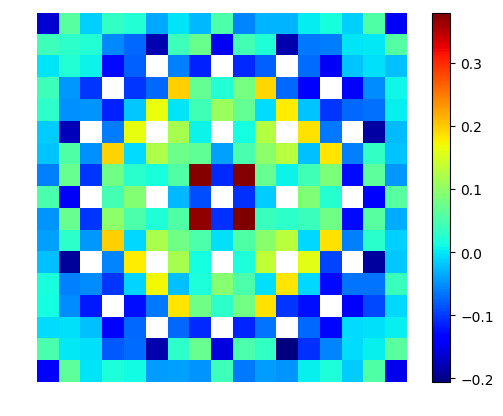
\includegraphics[width=\linewidth]{figures/assembly/fiss-null-errors}
  \caption{}
  \label{fig:assm-fiss-null-error}
\end{subfigure}%
\begin{subfigure}{0.45\textwidth}
  \centering
  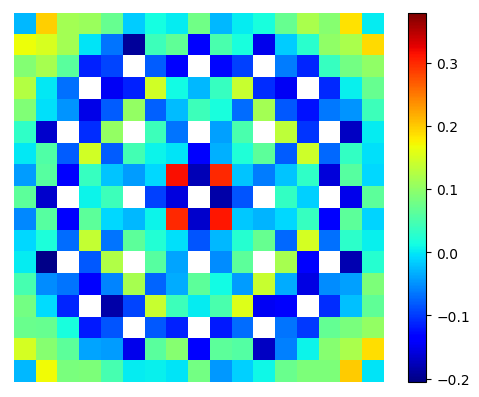
\includegraphics[width=\linewidth]{figures/assembly/fiss-degenerate-errors}
  \caption{}
  \label{fig:assm-fiss-degen-error}
\end{subfigure}
\begin{subfigure}{0.45\textwidth}
  \centering
  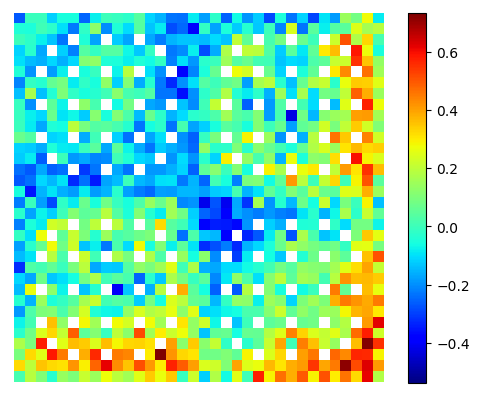
\includegraphics[width=\linewidth]{figures/reflector/fiss-null-errors}
  \caption{}
  \label{fig:reflector-fiss-null-error}
\end{subfigure}%
\begin{subfigure}{0.45\textwidth}
  \centering
  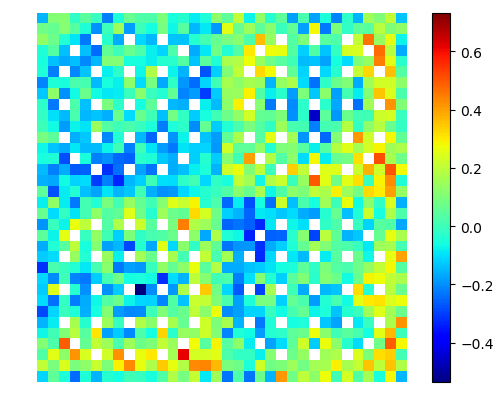
\includegraphics[width=\linewidth]{figures/reflector/fiss-degenerate-errors}
  \caption{}
  \label{fig:reflector-fiss-degen-error}
\end{subfigure}
\caption{OpenMOC fission rate percent relative errors for the (a) assembly and (b) 2$\times$2 colorset models.}
\label{fig:fiss-errors}
\end{figure*}


%%%%%%%%%%%%%%%%%%%%%%%%%%%%%%%%%%%%%%%%%%%%%%%%%%%%%%%%%%%%%%%%%%%%%%%%%%%%%%%
\subsection{Capture Rates}
\label{subsec:capt-rates}

-add figures of spatial distribution of errors

\begin{table}[h!]
  \centering
  \caption{OpenMOC U-238 capture rate percent relative errors.}
  \label{tab:capt-bias} 
  \begin{tabular}{l l r r}
  \toprule
  \textbf{Benchmark} & \textbf{Metric} & \textbf{Null} & \textbf{Degenerate} \\
  \midrule
  \multirow{2}{*}{Assembly} & Max  & -1.101 &  0.386 \\
                            & Mean &  0.479 &  0.086 \\
  \midrule
  \multirow{2}{*}{Colorset} & Max  & -1.969 & -0.783 \\
                            & Mean &  0.478 &  0.165 \\
  \bottomrule
\end{tabular}
\end{table}

\begin{figure*}[h!]
\centering
\begin{subfigure}{0.45\textwidth}
  \centering
  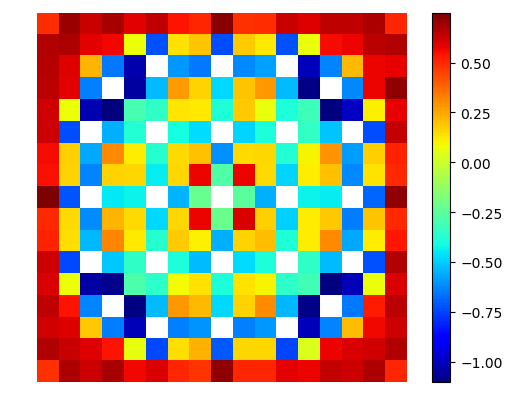
\includegraphics[width=\linewidth]{figures/assembly/capt-null-errors}
  \caption{}
  \label{fig:assm-capt-null-error}
\end{subfigure}%
\begin{subfigure}{0.45\textwidth}
  \centering
  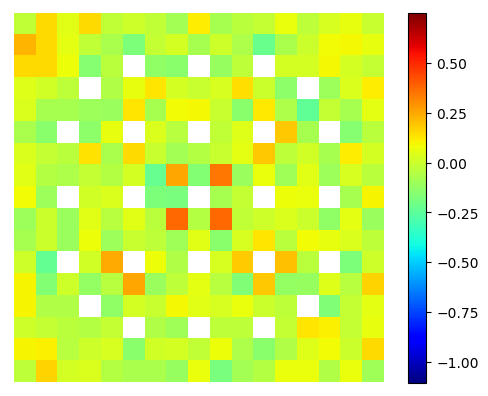
\includegraphics[width=\linewidth]{figures/assembly/capt-degenerate-errors}
  \caption{}
  \label{fig:assm-capt-degen-error}
\end{subfigure}
\begin{subfigure}{0.45\textwidth}
  \centering
  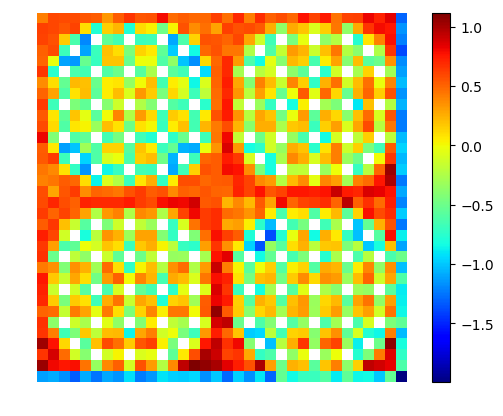
\includegraphics[width=\linewidth]{figures/reflector/capt-null-errors}
  \caption{}
  \label{fig:reflector-capt-null-error}
\end{subfigure}%
\begin{subfigure}{0.45\textwidth}
  \centering
  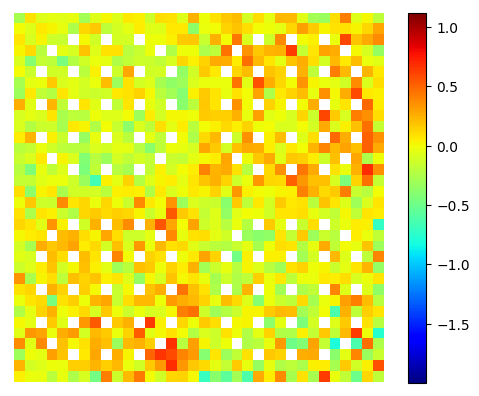
\includegraphics[width=\linewidth]{figures/reflector/capt-degenerate-errors}
  \caption{}
  \label{fig:reflector-capt-degen-error}
\end{subfigure}
\caption{OpenMOC U-238 capture rate percent relative errors for the (a) assembly and (b) 2$\times$2 colorset models.}
\label{fig:capt-errors}
\end{figure*}

